\documentclass[11pt]{article}
\usepackage[margin=1in]{geometry}
\usepackage{amsmath,amssymb}
\usepackage{booktabs}
\usepackage{graphicx}
\usepackage{enumitem}
\usepackage[hidelinks]{hyperref}
\usepackage{xcolor}
\hypersetup{colorlinks=true, linkcolor=blue!60!black, urlcolor=blue!60!black}

\newcommand{\Jh}{\hat{J}}

\title{Fix 2: Removing the Constant from the \texttt{msj} Energy}
\author{autotwin/automesh issue \#768}
\date{October 14, 2026}

\begin{document}
\maketitle

\section*{Summary}

Fix 2 subtracts $\Theta\,\ell^2$ from every hex's term in the \texttt{conspire} \texttt{msj} energy.
It does not change any step that L-BFGS takes.
It changes only the denominator of the stall test.
On the snapped bone octree at $\Theta = 0.32$, that denominator falls from 6,353.7 to $1.19 \times 10^{-3}$.
The stall test then reads full progress as full progress, and the ratchet continues from 0.319 to 0.470.

\section*{Notation}

$h$ is one hex, and $\ell(h)$ is its average edge length.
$\Jh(h)$ is the minimum scaled Jacobian of $h$ over its eight corners and its body center.
$\Theta \in [0, 1]$ is the current ratchet threshold for the minimum scaled Jacobian $\Jh$.
Each hex adds one term $\psi(h) = \ell^2 \min(\Jh, \Theta)$, the \texttt{conspire} form $\psi_{\mathrm{c}}$ of the companion HexOpt note.
The paper writes $\psi$ as $\mathit{ReHQJ}$, $\Jh$ as $\mathit{SJ}$, $\ell$ as $\bar{e}$, and $\mathcal{L}$ as $L$.
\texttt{improve} minimizes the augmented Lagrangian $\mathcal{L} = -\sum_h \psi(h)$ plus the terms that hold the boundary on the STL.
$\langle x \rangle = \max(x, 0)$ is the Macaulay bracket.
Within one ratchet level, $\Theta$ and every $\ell$ are fixed.

\section*{1. The stall test is a ratio}

After each L-BFGS run, \texttt{improve} computes
\begin{equation}
  \text{ratio} = \frac{\mathcal{L}_{\text{before}} - \mathcal{L}_{\text{after}}}{|\mathcal{L}_{\text{before}}|}
\end{equation}
and stops the level if the ratio is below $\texttt{STALL} = 10^{-6}$.
The numerator measures the work that the run did.
The denominator is meant to measure the work that remains.

\section*{2. The constant inflates only the denominator}

As shipped, a hex with $J > 0$ adds
\begin{equation}
  \psi(h) = \ell^2 \min\bigl(\Jh(h), \Theta\bigr) .
\end{equation}
Above $\Theta$, the term is the constant $\Theta\,\ell^2$.
No node move changes it, so it contributes nothing to the numerator.
It still sits in the denominator.

At $\Theta = 0.32$ on the octree, 9,266 hexes sit above $\Theta$.
Their constant terms sum to 6,353.4.
One hex sits below $\Theta$, and its term is 0.312.
The worst element is 0.3188, so its scaled Jacobian needs to rise by 0.0012 to meet $\Theta$.

Table~\ref{tab:run} gives the first L-BFGS run at this level, from the debug log.
The run lowers $\mathcal{L}$ by $1.19 \times 10^{-3}$, which is the full shortfall of the one hex.
Divided by 6,353.7, that drop gives a ratio of $1.9 \times 10^{-7}$.
The ratio is below $10^{-6}$, so \texttt{improve} stops the level.

\section*{3. Fix 2 removes the constant}

Fix 2 subtracts $\Theta\,\ell^2$ from every term.
Written as a per-hex energy that $\mathcal{L}$ sums directly, the result is
\begin{equation}
  w(h) = \Theta\,\ell^2 - \psi(h) = \ell^2 \, \bigl\langle \Theta - \Jh(h) \bigr\rangle ,
  \qquad
  \mathcal{L} = \sum_h w(h) + \text{boundary terms}.
\end{equation}
$w$ is nonnegative.
A hex above $\Theta$ adds exactly 0.
A hex below $\Theta$ adds its shortfall below $\Theta$, weighted by $\ell^2$.
The $J \le 0$ case shifts by the same constant, to $w = \Theta\,\ell^2 - J/\ell$.
Figure~\ref{fig:term} shows both forms of one hex's contribution to $\mathcal{L}$.
The two curves are parallel, offset by $\Theta\,\ell^2$.

\begin{figure}[h]
  \centering
  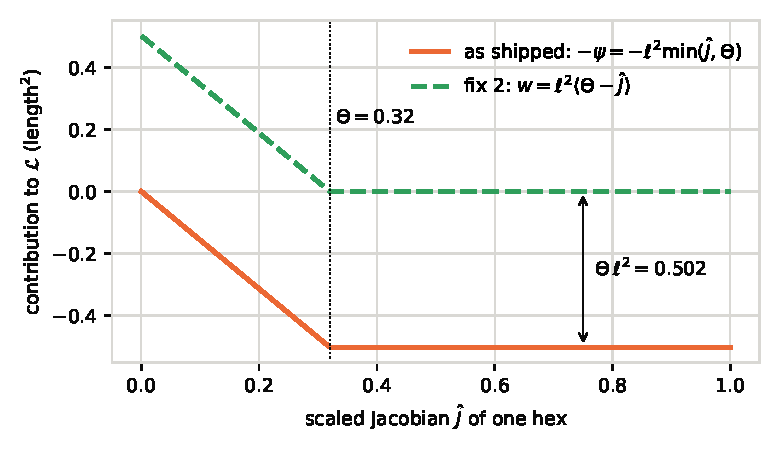
\includegraphics[width=0.75\textwidth]{fix2_term.pdf}
  \caption{One hex's contribution to $\mathcal{L}$, with $\ell = 1.253$, the median on the snapped octree, at $\Theta = 0.32$.
    As shipped (solid), $-\psi$ is flat at $-\Theta\,\ell^2 = -0.502$ above $\Theta$.
    With fix 2 (dashed), $w$ is flat at 0.
    Both have the same slope everywhere.}
  \label{fig:term}
\end{figure}

The hex part of $\mathcal{L}$ is now the total shortfall of all hexes below $\Theta$.
At $\Theta = 0.32$, the 6,353.4 disappears.
The same run now starts at $\mathcal{L} = 1.19 \times 10^{-3}$ and ends at $1.7 \times 10^{-24}$.
The ratio is 1.000, far above $10^{-6}$, so the level continues.

\begin{table}[h]
  \centering
  \begin{tabular}{lrr}
    \toprule
    first L-BFGS run at $\Theta = 0.32$ & as shipped & fix 2 \\
    \midrule
    worst element at start & 0.3188 & 0.3188 \\
    $\mathcal{L}_{\text{before}}$ & $-6{,}353.693$ & $1.186 \times 10^{-3}$ \\
    drop $\mathcal{L}_{\text{before}} - \mathcal{L}_{\text{after}}$ & $1.19 \times 10^{-3}$ & $1.19 \times 10^{-3}$ \\
    ratio & $1.9 \times 10^{-7}$ & 1.000 \\
    outcome & stops & continues \\
    \bottomrule
  \end{tabular}
  \caption{The same run, before and after fix 2, from the \texttt{msj} debug logs on the snapped octree.
    The drop matches to three digits.}
  \label{tab:run}
\end{table}

\begin{figure}[h]
  \centering
  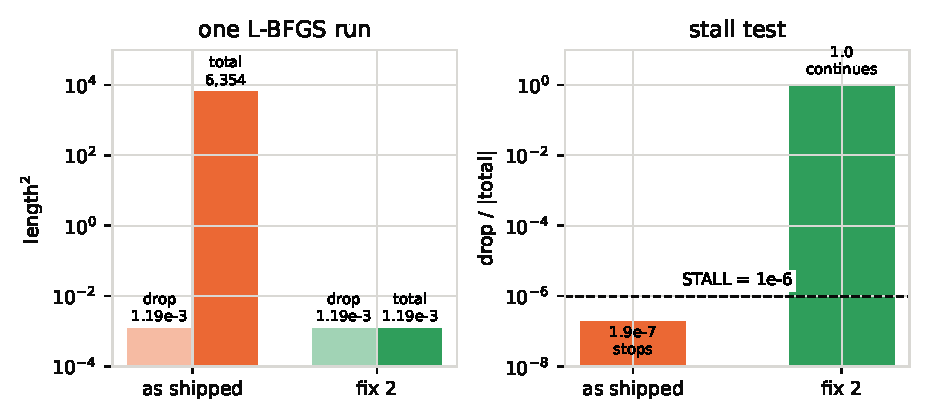
\includegraphics[width=0.9\textwidth]{fix2_ratio.pdf}
  \caption{Left: the drop and $|\mathcal{L}_{\text{before}}|$ for the run in Table~\ref{tab:run}, on a log scale.
    The drop is the same, and only the total changes.
    Right: the ratio against $\texttt{STALL} = 10^{-6}$ (dashed).}
  \label{fig:ratio}
\end{figure}

\section*{4. The steps do not change}

Within one level, $\Theta\,\ell^2$ is the same number before and after every node move.
Subtracting it leaves two things unchanged.
\begin{itemize}[leftmargin=*]
  \item \textbf{The gradient.}
    The derivative of a constant is zero, so $\nabla \mathcal{L}$ is the same.
    L-BFGS picks the same search direction.
  \item \textbf{Every energy difference.}
    The constant cancels in $\mathcal{L}(\text{new}) - \mathcal{L}(\text{old})$.
    The Armijo condition compares exactly this difference, so it accepts the same step lengths.
\end{itemize}
L-BFGS therefore takes the same path.
The drop in Table~\ref{tab:run} confirms this: $1.19 \times 10^{-3}$ in both columns.
Only the stall test sees a different number.

\section*{5. The effect on the ratchet}

Figure~\ref{fig:ratchet} shows the worst element at each accepted level on the octree.
As shipped, the ratchet accepts 2 levels and stops at 0.319.
With fixes 1 and 2, it accepts 18 levels and reaches 0.470.
It then stops at $\Theta = 0.48$ after all 20 sweeps of that level.
That limit is separate from the stall test.

\begin{figure}[h]
  \centering
  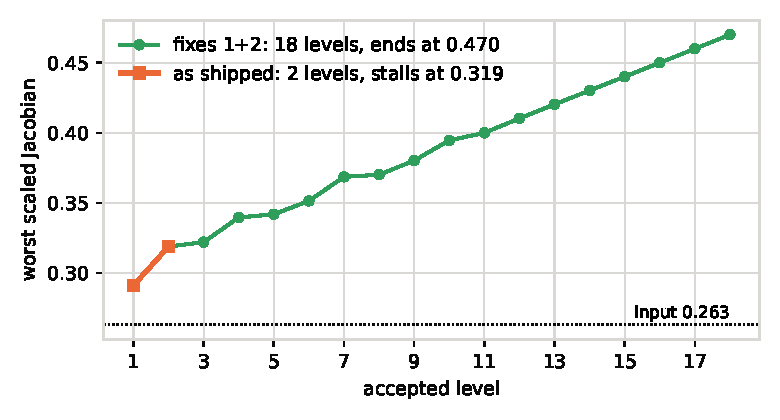
\includegraphics[width=0.75\textwidth]{fix2_ratchet.pdf}
  \caption{Worst scaled Jacobian at each accepted ratchet level on the snapped octree, from the debug logs.
    The dotted line is the input, 0.263.}
  \label{fig:ratchet}
\end{figure}

\section*{6. Why this matters beyond one mesh}

\begin{itemize}[leftmargin=*]
  \item \textbf{The constant grows with the mesh.}
    Each hex above $\Theta$ adds $\Theta\,\ell^2$.
    A mesh with ten times the hexes carries about ten times the constant.
    Lowering \texttt{STALL} to $10^{-9}$ moves the octree past 0.32, but a larger mesh would bring the stall back.
    Fix 2 removes the dependence on mesh size.
  \item \textbf{The energy has a direct meaning.}
    After fix 2, $\mathcal{L} = 0$ exactly when every hex meets $\Theta$.
    The value of $\mathcal{L}$ shows how much work remains.
\end{itemize}

\section*{7. What fix 2 does not address}

As the shortfall approaches 0, the ratio divides by a small number.
In the six runs on 2026-10-14, five of six ended by using all 20 sweeps of a level, not by the stall test.
These runs did not show the small-denominator case.

\end{document}
